% !TeX root = main.tex

\chapter{Heuristics}

In the previous chapter, we explored algorithms that found the exact closest pair.
However, at high dimensions, with millions of points, these algorithms become
computationally infeasible. The saving grace is that in many practical applications, we do
not always require the best answer, and can settle for something that is just \textit{good enough}.
As we shall see, even trying out many random pairs finds one that happens to be close to
the closest one. And we can also use simple principles to improve the quality of our guesses,
i.e., \textit{heuristics}. The downside of such techniques is that we cannot prove how
good or bad the final answer is, unlike \textit{approximation algorithms} where we put a limit
on the magnitude of the final error.

To judge the quality of a heuristic algorithm, we can measure how far off the discovered pair is
from the minimum distance. This needs to be handled carefully, however; the more iterations we run
of the random pair guessing algorithm, the more likely it is to get a better answer, so it is not
fair to buff a heuristic simply through stacking more guesses. Let us introduce the idea of a
\textit{budget}, so that each algorithm has a certain ``capacity'', which may be thought of as
a resource to be spent. The implication is that we can fix the budget, and attribute superior performance
to smarter ideas, rather than to more compute.

The most tempting approach would be to have this budget be \textit{runtime}, but empirically, it is not
that easy to figure out the set of parameters that yield a precise runtime. The alternative is
to go with a more theoretical construct, that is, the number of comparisons. Each comparison
is a distance computation between two points, and the budget is the number of comparisons you
perform per point, i.e., total comparisons over $n$. The budget is thus an integral
``multiple'' that is easy to work with. For simplicity, we define the budget rather loosely:
if you examine the same pair twice, it counts twice, and we exclude the cost of precomputations
from this budget, so you may perform sorting or build data structures free of charge. Of course,
the precomputations cannot be ludicrous; the ones used are all of subquadratic time.

\section{Random Pairs}

The simplest heuristic algorithm is born from a tiny modification to the brute force. At each
point, instead of trying every other one of the $n - 1$ points, we will pick a partner uniformly
at random and repeat this $a$ times (\code{attempts_per_point}). The budget is just $a$.

As seen in Figure~\ref{fig:heuristics_random_pairs}, the \textbf{ratio} (i.e., the distance found
divided by the true minimum distance) steadily decreases as we increase $a$. At $a = 60$,
we have found a pair whose distance is about $2.3$ times the closest distance. There
are diminishing returns to increasing $a$; going from $a = 6$ to $18$ improves the mean
by about as much as going from $18$ all the way to $60$. Luck is an important component
too; for each $a$, the ratio spread is pretty wide as we go from trial to trial,
and you could go anywhere from one to four at $a = 60$. Regardless, it is comforting
to know that examining just a tiny fraction of possible pairs already yields such a low ratio.

\begin{figure}[ht]
    \centering
    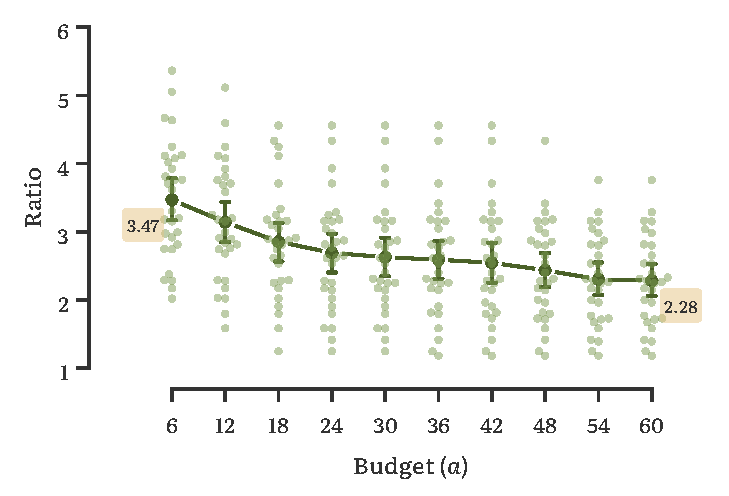
\includegraphics[scale=\figurescale]{diagrams/heuristics_random_pairs.pdf}
    \caption{Random pairs at $d = 6$ and $n = 10{,}000$.}
    \label{fig:heuristics_random_pairs}
\end{figure}

\section{Neighbours in a Sorted Order}

Sorting is the basis of the divide-and-conquer and sweepline algorithms. The reason they do not
scale to high dimensions is that the ``box'' of valid neighbours grows exponentially with $d$.
Nevertheless, there are different heuristics we may use to sort the points, the goal being
to place points that are close to each other near one another in the sorted order.

\subsection{Along Each Axis}

The first idea that comes to mind is to sort the points using their coordinate on one axis,
and then apply a sliding window, i.e., check $w$ neighbours per point. Intuitively, a closest pair
should be close on some axis (though there are counterexamples to refute this), and in total we
have a budget of $d \cdot w$.

\subsection{Along Random Directions}

To generalise the earlier idea, we can actually create our own axis (so we unlock
an arbitrary number of directions to sort by). First, let us pick some direction 
$u$ in $d$-dimensional space. Each component of $u$ is drawn independently from a standard normal
distribution, which makes the direction uniformly random over all directions~\cite{muller1959}.
Next, every point $p$ gets a sort key equal to the \textit{projection} $p \cdot u$. The
total budget is $m \cdot w$ (where $m$ is captured by \code{direction_count}).

\begin{figure}[ht]
    \centering
    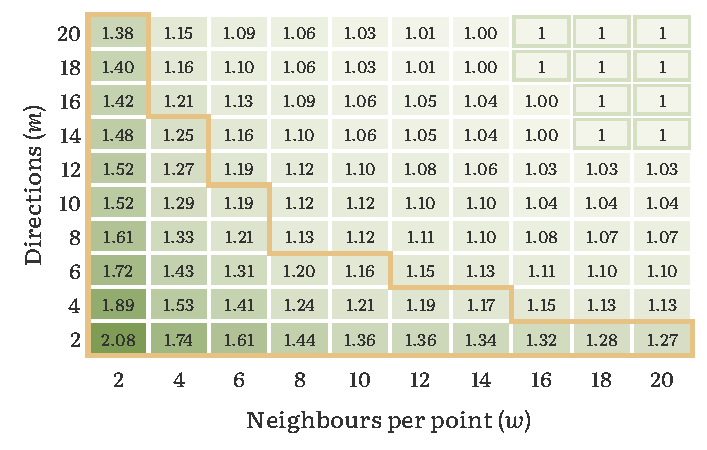
\includegraphics[scale=\figurescale]{diagrams/heuristics_random_directions.pdf}
    \caption{Mean ratio of random directions at $d = 6$ and $n = 10{,}000$; the yellow-bordered
        zone represents cells where $m \cdot w \leq 60$. Cells marked $1$ found the
        distance of the closest pair in \textit{every} trial.
    }
    \label{fig:heuristics_random_directions}
\end{figure}

As Figure~\ref{fig:heuristics_random_directions} shows, sorting is truly a powerful tool. Even
at a budget of four, we have already surpassed the best ratio random pairs had to offer at a budget
of sixty. In fact, given a maximum budget of sixty, trying random directions nets us a best ratio
of $1.16$.

Between $m$ and $w$, $w$ appears to have a slightly larger contribution, but that is
not to say $m$ is useless, because trying more directions reduces the risk of unlucky projections.
Another noteworthy observation is that at a budget of around three hundred, we are even able to
find the global minimum.

\subsection{Along the Z-order Curve}

An unorthodox way to sort would be through the Z-order curve (or Morton order~\cite{morton1966}).
This is a path that goes through every cell of a grid, and it forms a Z shape, giving it its
name. A point's position on the curve comes from \textit{interleaving} the bits of its coordinates:
starting from the topmost bit, you take one bit from each axis in turn. For example, $x = 101_{2}$
and $y = 011_{2}$ interleave to $100111_{2}$.

\begin{figure}[ht]
    \centering
    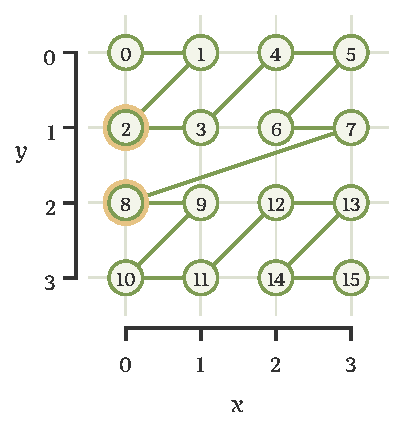
\includegraphics[scale=\figurescale]{diagrams/heuristics_z_order.pdf}
    \caption{The Z-order curve on a $4 \times 4$ grid. The two highlighted points are close on the
        grid, but far apart on the curve.
    }
    \label{fig:heuristics_z_order}
\end{figure}

\begin{aside}
    The most direct method to compare two points is to literally build the interleaved value.
    Since coordinates take up to $30$ bits, the resulting value would have $30 \cdot d$ bits,
    which does not fit in native types for many $d$. However, we only really care about
    the highest bit where the two points differ; a trick to check whether $x$ has a lower top
    bit than $y$ (\code{has_lower_most_significant_bit}) is to test $x < y$ and
    $x < x \oplus y$, where $\oplus$ is bitwise exclusive-or~\cite{chan2002}.
\end{aside}

As is evident from Figure~\ref{fig:heuristics_z_order}, points $\bigl(\begin{smallmatrix} 0 \\ 1 \end{smallmatrix}\bigr)$
and $\bigl(\begin{smallmatrix} 0 \\ 2 \end{smallmatrix}\bigr)$ are
close in terms of Euclidean distance, but when inspected in Morton order, they end up far
apart. One remedy is to apply a random shift to every point, creating a new order in the process.
Implementation-wise, we refrain from adding a shift to the very first order; only later orders
get a fresh shift, applied independently to each axis. With $s$ orders, we have a total budget
of $s \cdot w$.

\begin{figure}[ht]
    \centering
    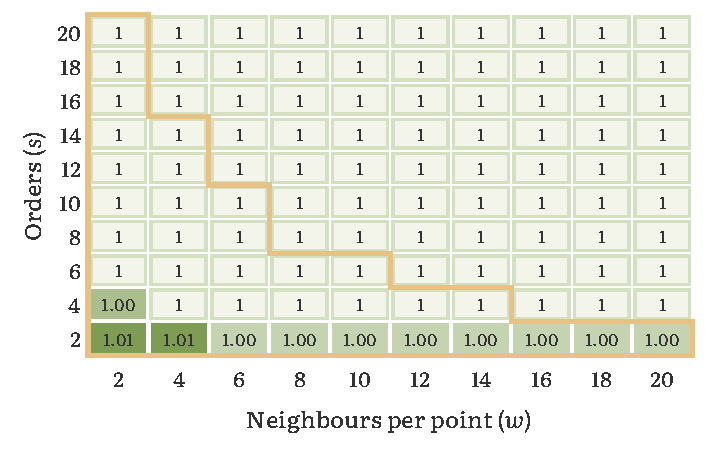
\includegraphics[scale=\figurescale]{diagrams/heuristics_z_order_heatmap.pdf}
    \caption{Mean ratio of the Z-order curve at $d = 6$ and $n = 10{,}000$; the yellow-bordered
        zone represents cells where $s \cdot w \leq 60$.
    }
    \label{fig:heuristics_z_order_heatmap}
\end{figure}

The Z-order curve is staggeringly impressive. Figure~\ref{fig:heuristics_z_order_heatmap} reveals
that across almost the entire budget spectrum, the closest pair was found \textit{thirty out of thirty}
times. Only with the fewest orders does the Z-order curve sometimes trip up and find a slightly
suboptimal pair.

\section{Best-first Search on the $k$-dimensional Tree}

In light of the success of the $k$-dimensional tree in the previous chapter,
it seems plausible that we could exploit the structure of the tree to reach nearby
points early in the traversal. Let us test out this
hypothesis by limiting the number of nodes traversed per query to just $b$. To pick the nodes
for expansion, we can use a Dijkstra-like approach (i.e., a best-first search) with
a min-heap. The budget is just $b$.

\begin{figure}[ht]
    \centering
    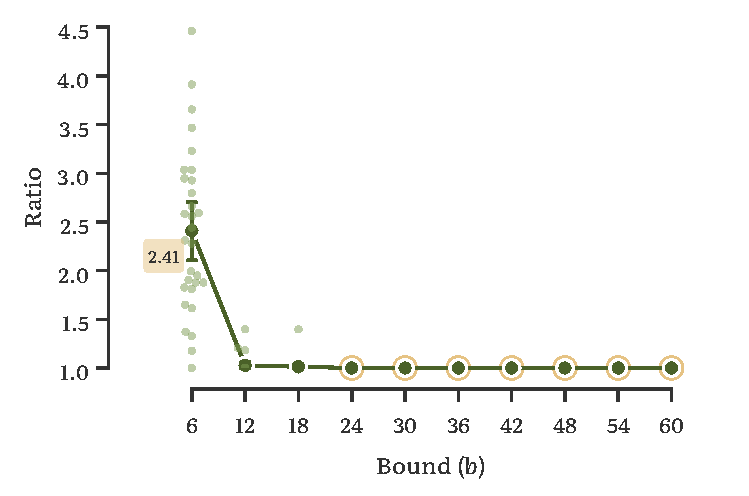
\includegraphics[scale=\figurescale]{diagrams/heuristics_best_first.pdf}
    \caption{Best-first search at $d = 6$ and $n = 10{,}000$; yellow rings mark the bounds where
        \textit{every} trial found the distance of the closest pair.
    }
    \label{fig:heuristics_best_first}
\end{figure}

It is apparent from Figure~\ref{fig:heuristics_best_first} that the results are on par
with the Z-order curve. At $b = 6$, the ratio is not particularly
great, but that is because traversal always begins from the root, regardless of the
query, and there will always be a few ``wasted nodes'' that cannot be avoided as part
of the expansion process. Nevertheless, from $b = 24$ onwards, it consistently
discovers the closest pair.

\section{High Dimensions}

As helpful as the ratio has been in our earlier benchmarking process, this metric
begins to lose its effectiveness at higher dimensions. At low dimensions, our best
heuristic algorithms are getting perfect scores, and at high dimensions, we are
\textit{also} getting near-perfect scores, which should raise some suspicions. The
reason is that the distribution of pair distances begins to contract as we increase the
number of dimensions, and even random pairs yield tiny ratios at high dimensions
(Figure~\ref{fig:heuristics_high_dimensions}).

\begin{figure}[ht]
    \centering
    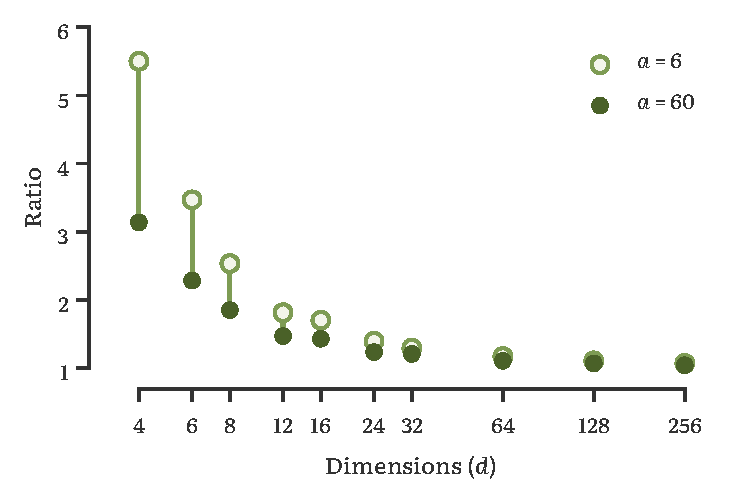
\includegraphics[scale=\figurescale]{diagrams/heuristics_high_dimensions.pdf}
    \caption{Mean ratio of random pairs at $n = 10{,}000$ as $d$ grows, at $a = 6$
        and $a = 60$.
    }
    \label{fig:heuristics_high_dimensions}
\end{figure}

Because the ratio only compares our pair with the closest pair, it fails to carry any information
about the underlying distribution. As $d$ grows, almost all pairs are about equally far apart,
a phenomenon known as \textit{distance concentration}~\cite{beyer1999}. He et al.\ measure this with
\textit{relative contrast}: the mean distance from a query to the data, divided by the distance
to its nearest neighbour~\cite{he2012}. Building on this idea, let $\delta$ be the distance
of the closest pair, $t$ be the mean distance over all pairs, and $x$ be the distance of a
candidate pair. We define the normalised score as:

\[
    S = \frac{t - x}{t - \delta}
\]

Visualise it as a ruler; your average pair lies at $0$ and the closest pair at $1$. This metric
does have a weakness, however, in that at low dimensions, because the ``ruler'' is incredibly
long, almost any pair scores pretty well.

As anticipated, Figure~\ref{fig:heuristics_comparison} reveals that even the strongest heuristic
algorithms have their limits. Performance-wise, the Z-order curve and best-first search are clearly
the (tied) winners. Random directions holds its own at $d \leq 8$, but its normalised score plummets
after that. There are three trends worth noticing. First, the normalised score tends to decrease
across the board as $d$ increases; as we enter sparse territory it becomes harder to leverage
data structures or representations that put close points beside each other. Second, the
\textit{variance} of the normalised score also rises with $d$ before levelling off at around
$d = 64$, i.e., it becomes harder to hit the mean score consistently. Finally, all four techniques appear
to converge to the same performance eventually. At super high dimensions, ``cleverness'' does not help
much and you are no better off than just trying random pairs. As pessimistic as it sounds, 
heuristics still have real value in commonly encountered dimensions. After all, it is not often one
needs to work with $2048$ dimensions,
and even at convergence, getting $90\%$ of the way there by examining about $2.6\%$ of the pairs is still
worth the compute.

\begin{figure}[ht]
    \centering
    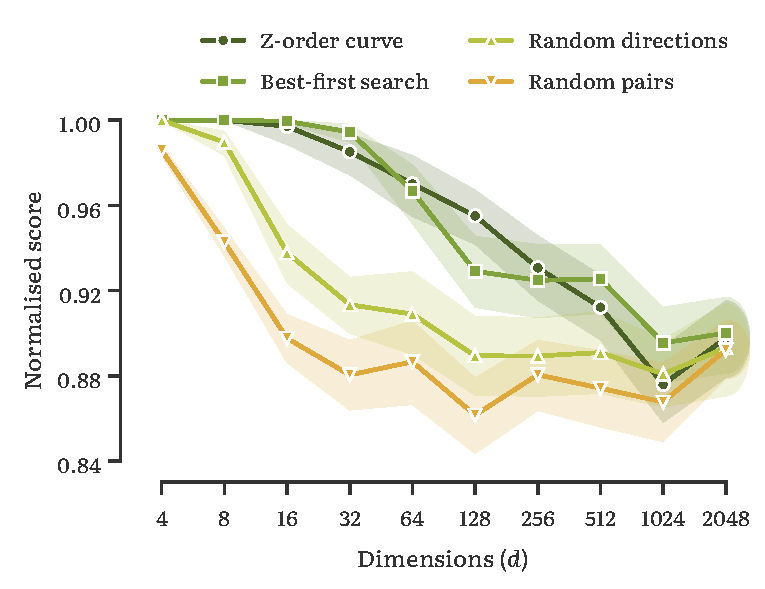
\includegraphics[scale=\figurescale]{diagrams/heuristics_comparison.pdf}
    \caption{Mean normalised score at a budget of $128$ and $n = 10{,}000$, using $s = 8$, $w = 16$ for
        the Z-order curve, $b = 128$ for best-first search, $m = 8$, $w = 16$ for random directions,
        and $a = 128$ for random pairs. Shaded bands show the 95\% confidence interval of each mean.
    }
    \label{fig:heuristics_comparison}
\end{figure}

